\section{Introduction}
	\paragraph{}{
	This chapter will outline the implementation and testing process adopted during the project. This will include information on how each component was implemented as well as any issues that occurred during the project and how they were resolved.
	}
\section{Development Environment}
	\paragraph{}{%Win10, ECU, Jenkins
	Before starting implementation, a suitable development environment was required. This included a Windows 10 development PC and a method of simulating connection to a vehicle. 
	}
	\paragraph{}{
	A development PC running Windows 10 was required as part of the development environment. It was also preferable that the PC had a touchscreen, to allow testing of gesture controls, such as swipe and pinch, without deploying to a tablet. Fortunately, a Windows 8.1 touchscreen laptop which was eligible for a free Windows 10 upgrade was available before the project began. After the development PC was set up, research began on acquiring a Windows 10 tablet or phone to deploy the application on. However, at the time of setting up the development environment, no such devices were readily available.			
	}
	\paragraph{}{
	In order to be able to test the application, it needed to connect to and communicate with a vehicle. However, this was not practical as it would require moving from the development environment to the vehicle when testing or debugging the application. Initially, an application that simulated connection to an ECU was bought and used. However, during development it became evident that this would not be suitable for the project, as outlined in section 5.5.2.
	}
	\paragraph{}{
	Instead, an ECU test bench was created that could be used as part of the development environment. This consisted of an ECU from a Rover 75 with an OBDII port and a power supply. A specific wiring diagram for the ECU had to be acquired in order to connect the wires to the corresponding pins on the ECU and OBDII port. The ECU test bench can be expanded with additional ECUs to facilitate the testing of communications with multiple communication protocols and vehicle manufacturers.
	}
	\begin{figure}[h]
		\begin{center}										
				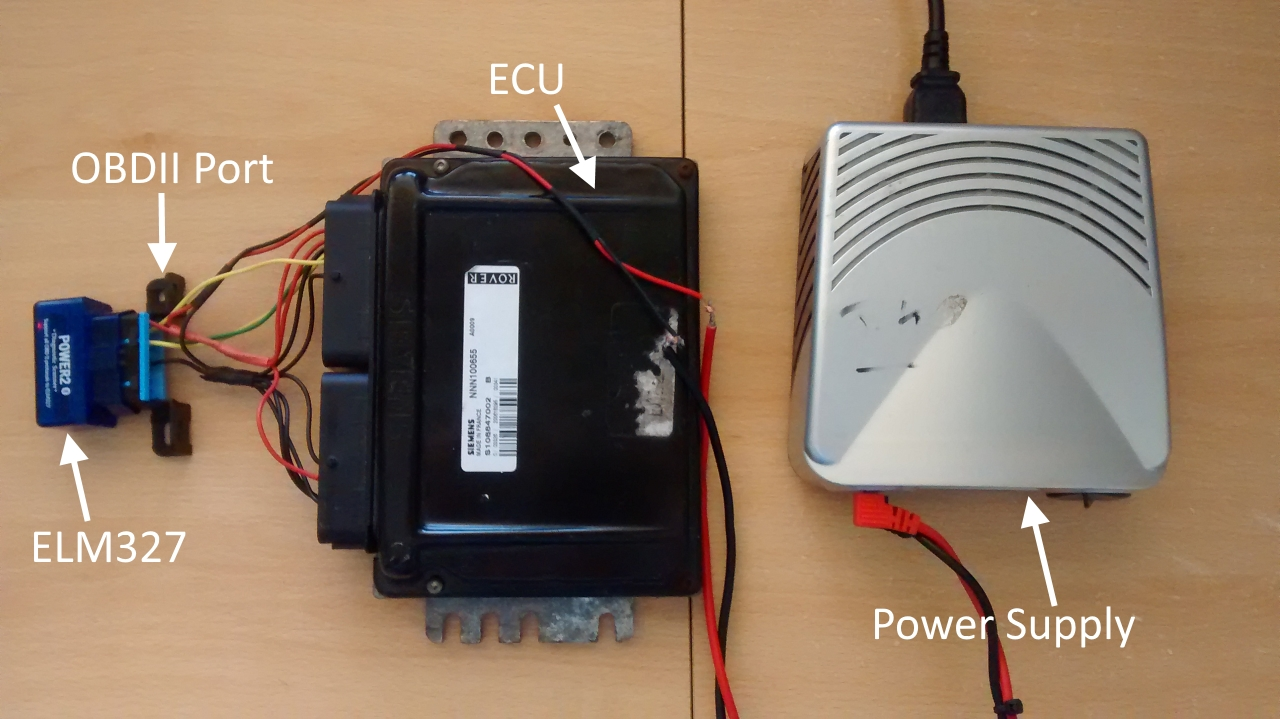
\includegraphics[width=0.9\textwidth]{ECUDesk.jpg}
				\caption{ECU test bench}
		\end{center}
	\end{figure}

\section{Prototyping}
	\paragraph{}{
	Prior to starting the project, a lightweight proof of concept was created. This was a C{\#} console application that could connect to an ELM327 simulation application, and display live data on the screen. 
	}
	\paragraph{}{ %Bluetooth API
	The application used the 32Feet API by In The Hand Ltd. to handle Bluetooth communication with the ELM327 simulator. The communication system was low level, as it required the address of the laptop and simulator to establish a connection. This was more low level than anticipated and resulted in the hard-coding of the addresses of the development laptop and simulator into the application, which was not optimal. One of the advantages of the 32Feet API, is that the developer can pair Bluetooth devices within their own application. However, this may also be a security issue as an incompatible or harmful device may be paired without the end user's knowledge.
	}
	\paragraph{}{
	The ELM327 simulation software used was an Android application called ECU Engine Pro. The application simulates an ELM327 device connected to an ECU using the CAN protocol. The user can manually add up to six DTCs, and can access the VIN and a limited number of PIDs, such as engine speed. The application displays the address to establish connection via Bluetooth, then the user is taken to the control panel, where they can monitor incoming and outgoing communication logs, as well as edit the DTCs and PID values being returned.
	}
	\paragraph{}{
	The application established communications with the simulator and configured the ELM327 device to use the CAN protocol using the pre-defined commands. The application would then display the first DTC as well as the current engine speed. The values that were displayed were the result of the formatting and converting of the raw data from the simulator. These conversions were hard-coded into the application, as there was only one PID that was being displayed.
	}
	\paragraph{}{	
	Overall, the prototype was a success, as it was able to display a DTC as well as the current engine speed on screen. This provided an insight into how communication and data conversion was handled, as well as how to configure the ELM327 device.
	}

\section{Implementation}
	\subsection{Bluetooth Communication}
		\paragraph{}{
		Implementation of the Bluetooth communication layer of the application began immediately after the setup of the development environment. The goal of this stage was to implement generic Bluetooth communication, such as establishing a connection with the ELM327 device and configuring it, rather than working on module specific communication, such as converting responses. The configuration steps involved resetting the device, allowing the device to auto-detect the communication protocol, turning off echoing of messages and allowing for long responses.
		}
		\paragraph{}{
		There were some issues with the 32Feet Bluetooth API, outlined in section 5.5.1, that lead to the use of Microsoft's own Bluetooth API in it's place. This API allows developers to find all Bluetooth device paired with the PC and choose the appropriate one from the list. Due to the use of this new API, there was less time to work on Bluetooth communication, so the application was created to connect to the first suitable Bluetooth device on the network, with the intention of adding a search function at a later date.
		}
		
	\subsection{DTC Module}
		\paragraph{}{
		Implementation of the DTC module involved creating a UI layer, a module layer and a communication layer for DTCs.	Initially, the DTC module was implemented to only retrieve and display one DTC of each type. This was to quickly test the functionality of the communication system and to provide an impression of the general aesthetics of the module, before implementing it in its entirety.
		}		
		\paragraph{}{
		The core functionality of this module was to request all current, pending and permanent DTCs and display them on screen grouped by their types. Initially, the module requested current DTCs, and only converted and displayed the first DTC from the response. This code was then reworked to display the first pending DTC and the first permanent DTC. Once the user interface was fully implemented, the module was rewritten to display all DTCs.
		}
		\paragraph{}{
		Another key aspect of this module was the implementation of the clear codes functionality. The module included a button that, when pressed, issued the clear codes command, then acquired the new list of DTCs and refreshed the UI.
		}
		
\section{Issues}
	\paragraph{}{
	During implementation, a number of serious issues were encountered that affected the design and development of the project. These issues were resolved, but often required a reconsideration of the initial design decisions.
	}
	
	\subsection{Issue 1: Bluetooth API}
		\paragraph{Description:}{
		The 32Feet Bluetooth API used in the prototype was incompatible with the UWP application. This meant that the prototype code that was written for Bluetooth connection could not be reused in the final product.
		}
		\paragraph{Occurred during:}{
		Week 1
		}
		\paragraph{Time taken to resolve:}{
		Approximately one week
		}
		\paragraph{Attempts to resolve:}{
		A number of attempts to resolve the issue were made, such as searching for newer versions of the API and researching potential workarounds. Unfortunately, it became evident that the API was completely incompatible with UWP applications, leading to a stand still in development until a replacement could be found.
		}
		\paragraph{Solution:}{
		Microsoft includes their own Bluetooth API with UWP and this was chosen as a replacement for the 32Feet Bluetooth API. Aside from the unexpected learning curve, this solution had it's inconveniences, such as not allowing devices to be paired through the application. This meant that there was additional configuration required by the end user. However, this also created a more secure application, as the chance of automatically pairing a potentially malicious device was decreased.
		}
	\subsection{Issue 2: Simulation software}
		\paragraph{Description:}{
		The replacement Bluetooth API could not connect to the ECU simulation software. This meant connection to an actual vehicle was required to debug and test the application.
		}
		\paragraph{Occurred during:}{
		Week 1
		}
		\paragraph{Time taken to resolve:}{
		Approximately two weeks
		}
		\paragraph{Attempts to resolve:}{
		Several attempts to contact the developer were made through emails and the Google Play Store, where the application was bought. Unfortunately, no response was received and a decision was reached that the application could not be utilised for this project, as it seemed highly unlikely that the application would be updated to support the Bluetooth API. 
		}
		\paragraph{Solution:}{
		To simulate connection to a vehicle, an ECU test bench was created as outlined in section 5.2. This had an impact on the timeline of the project, as a number of components, such as an ECU and a wiring diagram, had to be sourced as well as assembling the test bench itself. Ultimately, the ECU test bench had the advantage of extensibility over the ECU simulation software, as the latter only supported one protocol, whereas the former can be extended with new ECUs that support various protocols.
		}
	
\section{Testing}
	\paragraph{}{
	Testing of the application is essential in ensuring that the system satisfies the functional and non-functional requirements.
	}
	\paragraph{}{
	Ensuring the application displays the correct data is paramount, as an erroneous data value could cause confusion for the end user. Functional testing will ensure that data is not incorrectly converted by the communication system or incorrectly displayed by the UI. The output of the application will be compared with the output of the similar applications outlined in section 2.4, to ensure there is no disparity. 
	}
	\paragraph{}{
	Unit tests will be written for each component of the application. These unit tests will be run before a change is ready to be committed to the source control repository. If any unit tests fail, that have not failed prior to the implementation of the recent changes, the code will not be committed until the underlying causes have been fixed. This helps to minimise the number of new defects introduced as part of implementing new features.
	}